\chapter{Interaction of photons with matter}

\begin{figure}[tb]
\centering
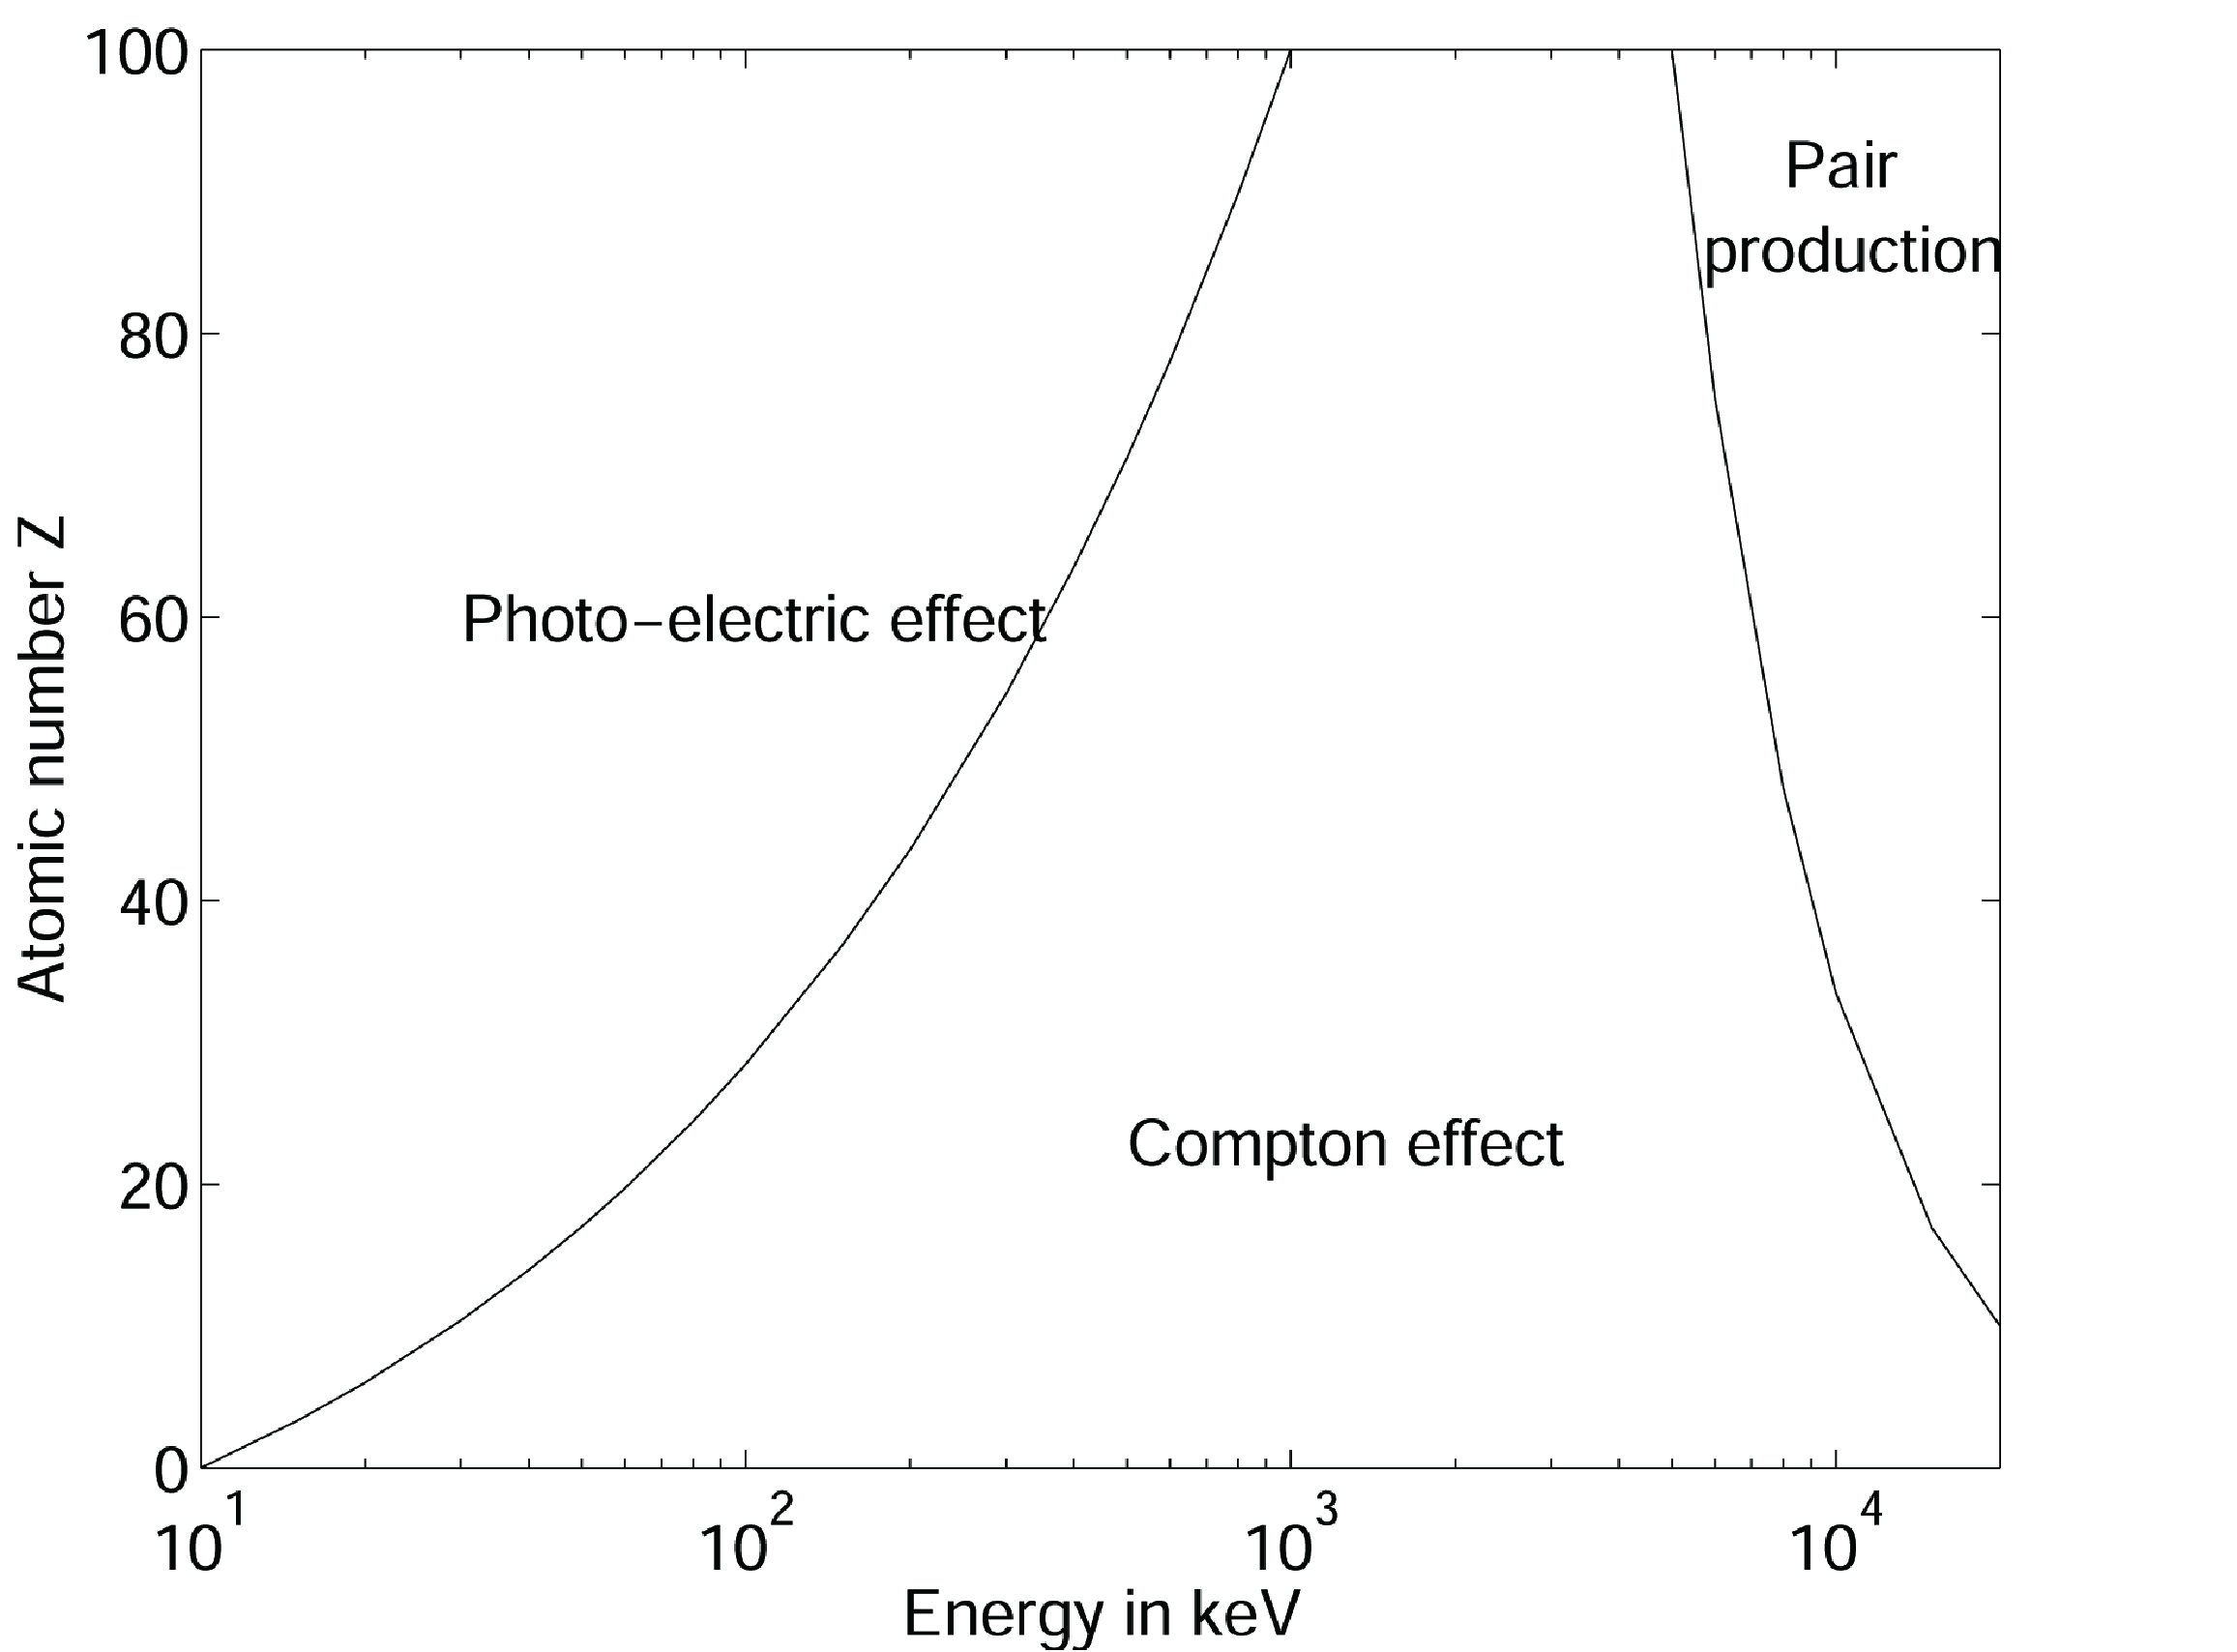
\includegraphics[width = \figone]{fig_foto_compton_pair.eps}
\caption{\label{fig:foto_compton_pair} \emph{Dominating interaction as a
function of electron number Z and photon energy.}}
\end{figure}

In nuclear medicine, photon energy ranges roughly from 60 to 600 keV. For
example, \Tc\ has an energy of 140 keV. This corresponds to a wave
length of 9~pm and a frequency of 3.4 $\times$ $10^{19}$ Hz. At such energies,
$\gamma$ photons behave like particles rather than like waves.

At these energies, the dominating interactions of photons with matter are
photon-electron interactions: Compton scatter and photo-electric effect. As
shown in figure \ref{fig:foto_compton_pair}, the dominating interaction is a
function of energy and electron number. For typical nuclear medicine
energies, Compton scatter dominates in light materials (such as water and
human tissue), and photo-electric effect dominates in high density materials.
Pair production (conversion of a photon in an electron and a positron) is
excluded for energies below 1022 keV, since each of the particles has a mass
of 511 keV. Rayleigh scatter (absorption and re-emission of (all or a
fraction of) the absorbed energy as a photon in a different direction) has a
low probability.

\section{Photo-electric effect}
%%%%%%%%%%%%%%%%%%%%%%%%%%%%%%%%%
A photon ``hits'' an electron, usually from an inner shell (strong
binding energy). The electron absorbs all the energy of the photon. If
that energy is higher than the binding energy of the electron, the
electron escapes from its atom. Its kinetic energy is the difference
between the absorbed energy and the binding energy. In a dense
material, this photo-electron will collide with electrons from other
atoms, and will lose energy in each collision, until no kinetic energy
is left.

As a result, there is now a electron vacancy in the atom, which may be filled
by an electron from a higher energy state. The difference in binding energy
of the two states must be released. This can be done by emitting a photon.
Alternatively, the energy can be used by another electron with low binding
energy to escape from the atom.

In both cases, the photon is completely eliminated.

The probability of a photo-electric interaction is approximately proportional
to $Z^3 / E^3$, where $Z$ is the atomic number of the material, and $E$ is the
energy of the photon. So the photo-electric effect is particularly important for
low energy radiation and for dense materials.

\section{Compton scatter \label{sec:compton_scatter}}
%%%%%%%%%%%%%%%%%%%%%%%%%%%%%%%%%%%%%%%%%%%%%%%%%%%%%
\begin{figure}[tb]
\centering
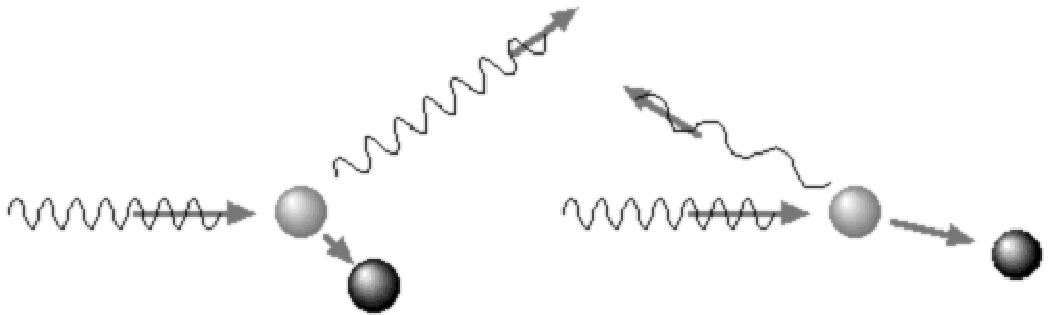
\includegraphics[width=\figone]{fig_compton_scatter.eps}
\caption{\label{fig:compton_scatter} \emph{Compton scatter can be regarded as
an elastic collision between a photon and an electron.}}
\end{figure}

Compton scatter can be regarded as an elastic collision between a
photon and an electron. This occurs with loosely bound electrons
(outer shell), which have a binding energy that is negligible compared
to the energy of the incident photon. The term ``elastic'' means that
total kinetic energy before and after collision is the same. As in any
collision, the momentum is preserved as well. Applying equations for
the conservation of momentum and energy (with relativistic
corrections) results in the following relation between the photon
energy before and after the collision:
\begin{equation}
  E'_\gamma \;\;=\;\; E_\gamma \frac{1}{1 
     + \Frac{E_\gamma}{m_e c^2} (1 - \cos\theta)} \label{eq:jn_compton_energy}
   \;\; = \;\; E_\gamma \; P(E_\gamma, \theta)
\end{equation}
%
$\begin{array}{llrl}
\mbox{with}
            & E'_\gamma & = & \mbox{energy after collision}\\
            & E_\gamma  & = & \mbox{energy before collision}\\
            & m_e       & = & \mbox{electron rest mass}\\
            & \theta    & = & \mbox{scatter angle}
\end{array}$\\
%
The expression $m_e c^2$ is the energy available in the mass of the
electron, which equals 511 keV. For a scatter angle $\theta$ = 0, the
photon loses no energy and it is not deviated from its original
direction: nothing happened.  The loss of energy increases with
$\theta$ and is maximum for an angle of 180\degrees. The probability
that a photon will interact at all with an electron depends on the
energy of the photon. If the interaction takes place, each scatter
angle has its own probability, and this probability is proportional to
the differential cross section, given by the Klein-Nishina equation:
\begin{equation}
 \frac{d\sigma}{d\Omega} = \frac{1}{2} r_e^2 \; P(E_\gamma, \theta)^2
    \left( P(E_\gamma, \theta) + \frac{1}{P(E_\gamma, \theta)} - \sin^2\theta \right),
    \label{eq:kleinnishina}
\end{equation}
where $r_e$ is the classical electron radius and $P(E_\gamma, \theta)$
is defined above. The cross section $\sigma$ has the unit of area,
$\Omega$ is the solid angle. Integrating over $\Omega$
would produce the total cross section for Compton scatter. For that
integration, $d\Omega$ can be written as $2 \pi \sin\theta \,d\theta$
\footnote{If you are not sure why, this is explained in the derivation
  of equation (\pref{eq:wellcounter}).}.
The differential cross section (\ref{eq:kleinnishina}) is shown for a
few incoming photon energies in figure \ref{fig:kleinnishina}. For
higher energies, smaller scatter angles become increasingly likely.

\begin{figure}[htb]
\centering
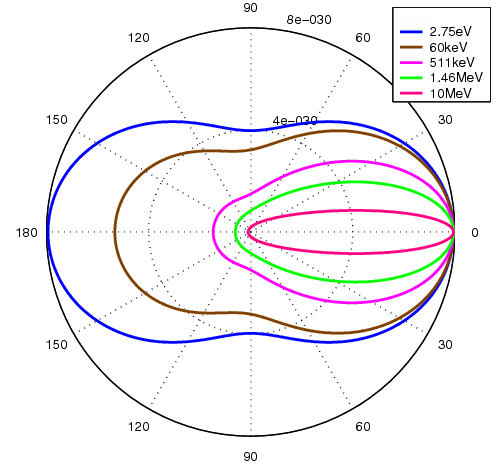
\includegraphics[bb=0 0 500 473,width=\figmedium]{fig_klein_nishina.png}
\caption{\label{fig:kleinnishina} \emph{The scattering-angle
    distribution for a few photon energies. Figure from Wikipedia
    (https://en.wikipedia.org/wiki/Klein-Nishina\_formula).}}
\end{figure}


The probability of a Compton decreases very slowly with increasing $E$
(see fig. \ref{fig:atten_water}) and with increasing $Z$.

Because the energy of the photon after scattering is less than before,
Compton scatter is sometimes also called ``inelastic scattering''.

\section{Rayleigh scatter}
%%%%%%%%%%%%%%%%%%%%%
Rayleigh scattering or coherent scattering can be regarded as the
collision between a photon and an entire atom. Because of the huge
mass of the atom, the photon is deflected from its original trajectory
without any noticeable loss of energy (replace $m_e c^2$ with $\infty$
in (\ref{eq:jn_compton_energy})). Rayleigh scattering contributes only
significantly at low energies, and can be safely ignored in typical nuclear
medicine applications. Because the energy of the photon after
scattering is the same as before, this effect is also called ``elastic
scattering''.

\section{Attenuation}
%%%%%%%%%%%%%%%%%%%%%

\begin{figure}[tb]
\centering
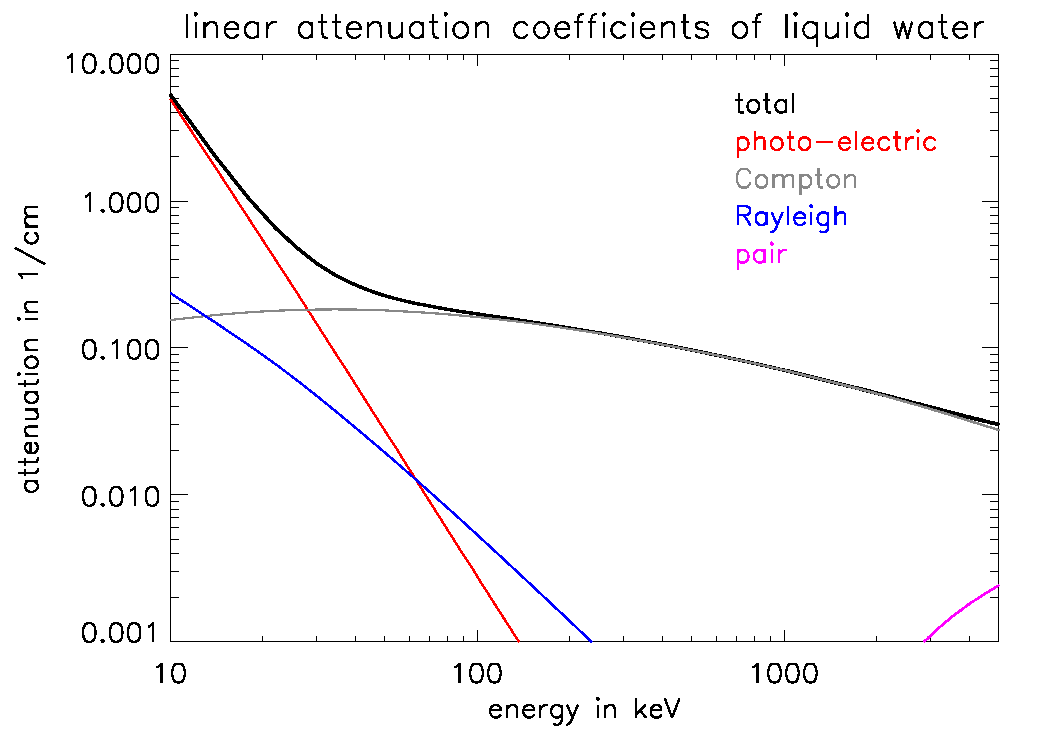
\includegraphics[width=\figmedium]{fig_atten_water.eps}
\caption{\label{fig:atten_water} \emph{Photon attenuation in water as a
function of photon energy. The photo-electric component decreases
approximately with $(Z/E)^3$ (of course, $Z$ is a constant here). The Compton
components varies slowly.}}
\end{figure}

The {\em linear attenuation coefficient} $\mu$ is defined as the
probability of interaction per unit length (unit: cm$^{-1}$). Figure
\ref{fig:atten_water} shows the mass attenuation coefficients as a
function of energy in water. Multiply the mass attenuation coefficient
with the mass density to obtain the linear attenuation
coefficient. When photons are traveling in a particular direction
through matter, their number will gradually decrease, since some of
them will interact with an electron and get absorbed (photo-electric
effect) or deviated (Compton scatter) into another direction. By
definition, the fraction that is eliminated over distance $ds$ equals
$\mu(s) N(s)$:
\begin{equation}
  dN(s) = - \mu(s) N(s) ds. \label{eq:diff_atten}
\end{equation}

If initially $N(a)$ photons are emitted in point $s = a$ along the $s$-axis,
the number of photons $N(d)$ we expect to arrive in the detector at position
$s = d$ is obtained by integrating (\ref{eq:diff_atten}):
\begin{equation}
  N(d) = N(a) \  e^{- \int_a^d \mu(s) ds}. 
\label{jn:spectatten}
\end{equation}
Obviously, the attenuation of a photon depends on where it has been emitted.

\begin{figure}[tb]
\centering
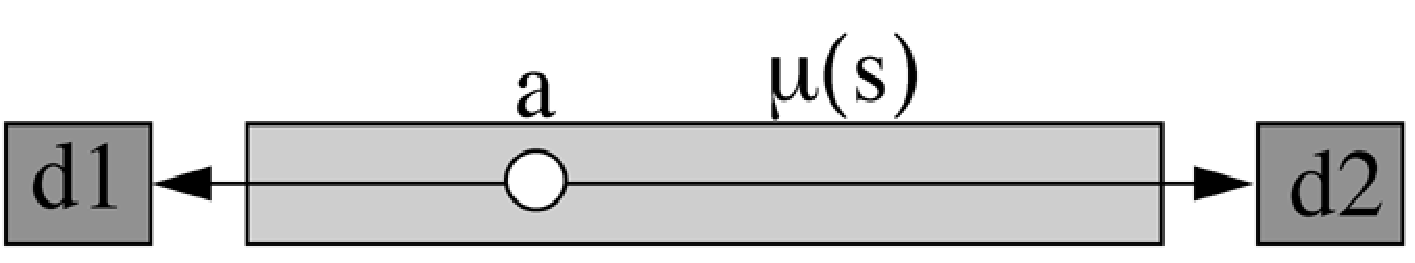
\includegraphics[width=\figone]{fig_jnpetatten.eps}
\caption{\label{fig:jn_petatten} \emph{Positron emitting point source in a
non-uniform attenuator.}}
\end{figure}
For positron emission, a pair of photons need to be detected. Since the fate
of both photons is independent, the detection probabilities must be
multiplied.  Assume that one detector is positioned in $s = d_1$, the second
one in $s = d_2$, and a point source in $s = a$, somewhere between the two
detectors. Assume further that during a measurement, $N(a)$ photon pairs were
emitted along the $s$-axis (fig.\ref{fig:jn_petatten}). The number of
detected pairs then is:
\begin{equation}
  N(d_1,d_2) = N(a)  e^{- \int_{d_1}^a \mu(s) ds} e^{- \int_a^{d_2} \mu(s)
             ds} \\
             = N(a)  e^{- \int_{d_1}^{d_2} \mu(s) ds}. \\
\label{jn:petatten}
\end{equation}
Equation (\ref{jn:petatten}) shows that for PET, the effect of attenuation is
independent of the position along the line of detection.

Photon-electron interactions will be more likely if there are more electrons
per unit length. So dense materials (with lots of electrons per atom) have a
high linear attenuation coefficient.